\documentclass[12pt, a4paper]{article}


\usepackage{arxiv}

\usepackage[utf8]{inputenc} % allow utf-8 input
\usepackage[T1]{fontenc}    % use 8-bit T1 fonts
\usepackage{hyperref}       % hyperlinks
\usepackage{url}            % simple URL typesetting
\usepackage{booktabs}       % professional-quality tables
\usepackage{amsfonts}       % blackboard math symbols
\usepackage{nicefrac}       % compact symbols for 1/2, etc.
\usepackage{microtype}      % microtypography
\usepackage{graphicx}
\graphicspath{{figures/}}
\usepackage[round]{natbib}
\setcitestyle{{aysep={}}}
\bibliographystyle{abbrvnat}
\usepackage{doi}
\usepackage{multirow}
\usepackage{caption}
\usepackage[nottoc]{tocbibind}
\usepackage[toc,title,page]{appendix}
\usepackage{minted}
\usepackage{neuralnetwork}
\usepackage{pgfplots}

\usepackage{tikz}
\usepackage{subcaption}
\pgfplotsset{compat=1.17}
\pgfplotsset{every axis/.append style={tick label style={/pgf/number format/fixed},font=\scriptsize,ylabel near ticks,xlabel near ticks,grid=major}}

\usepackage[braket, qm]{qcircuit}
\usepackage{amsmath}
\pdfmapfile{+sansmathaccent.map}

\usepackage{helvet}
\renewcommand{\familydefault}{\sfdefault}

\rfoot{33225857}

\title{Classical-quantum neural networks and varying numbers of qubits}

\date{2021}

\author{ {\hspace{1mm}33225857 (Daniel Duncan)} \\ % remove name from final
	Science Extension \\
	Northern Beaches Secondary College Manly Campus \\
	Sydney, NSW 2099 \\
	\texttt{} \\ % email
}

\renewcommand{\undertitle}{Draft}

%%% Add PDF metadata to help others organize their library
%%% Once the PDF is generated, you can check the metadata with
%%% $ pdfinfo template.pdf
\hypersetup{
pdftitle={Artificial Classical-Quantum Neural Networks and Varying Numbers of Qubits},
% not sure about subject tag
pdfsubject={cs.ET},
pdfauthor={Daniel J. Duncan},
pdfkeywords={First keyword, Second keyword, More},
}

\begin{document}
\maketitle

\begin{abstract}
+why the research is important\\
To determine the effect of the number of qubits employed in the quantum layer of a quantum-classical neural network on its classification accuracy, code from the Qiskit textbook was run on the IBM quantum computer ibmq\_manila, and the number of qubits employed by the network was varied from 1 to 5.
\\+what results were, what they indicated, whether they supported hypothesis

\end{abstract}

\tableofcontents

\newpage
\section{Literature Review}
As quantum computing becomes increasingly viable, its applications must be examined. A technology which may benefit from quantum computer acceleration is neural networks. In a review of progress made in the field of machine learning (ML) and quantum physics, and quantum machine learning (QML), applying ML to quantum physics, mainly involving quantum mechanical calculations which are traditionally difficult to complete, and quantum enhancements for ML and the potential speedup of various tasks are explored \citep{Dunjko2018}. Despite the capabilities of quantum computers being rapidly expanded by innovations in both quantum hardware, and algorithms for the software executed on them, they remain simplistic. Quantum computers are currently noisy intermediate scale quantum (NISQ) technologies. \emph{"Intermediate scale [describes] devices that are large enough ... that we can't by brute force simulate the quantum system using our most powerful existing digital computers … noisy reminds us that the ... quantum gates in the device will sometimes make errors ... so noise is going to limit their computational power"} \citep{preskill}. Noise and scale related limitations of computational power mean that purely quantum neural networks are difficult to implement and test, but hybrid classical-quantum neural networks are viable.

\subsection{Quantum Computing}
In Simulating Physics with Computers \citep{Feynman1982}, Richard Feynman proposed that in order to simulate the exact physics of nature, quantum physics must be perfectly modelled using a computer which is fundamentally quantum. Like classical computers, quantum computers receive an input, do processing, and then return an output. Unlike classical computers which use bits, quantum computers make use of qubits (quantum bits). Qubits are fundamentally quantum objects (atoms, ions and photons), and can be represented as a Bloch sphere (figure \ref{fig:bloch_sphere}).
\begin{figure}[h]
    \centering
    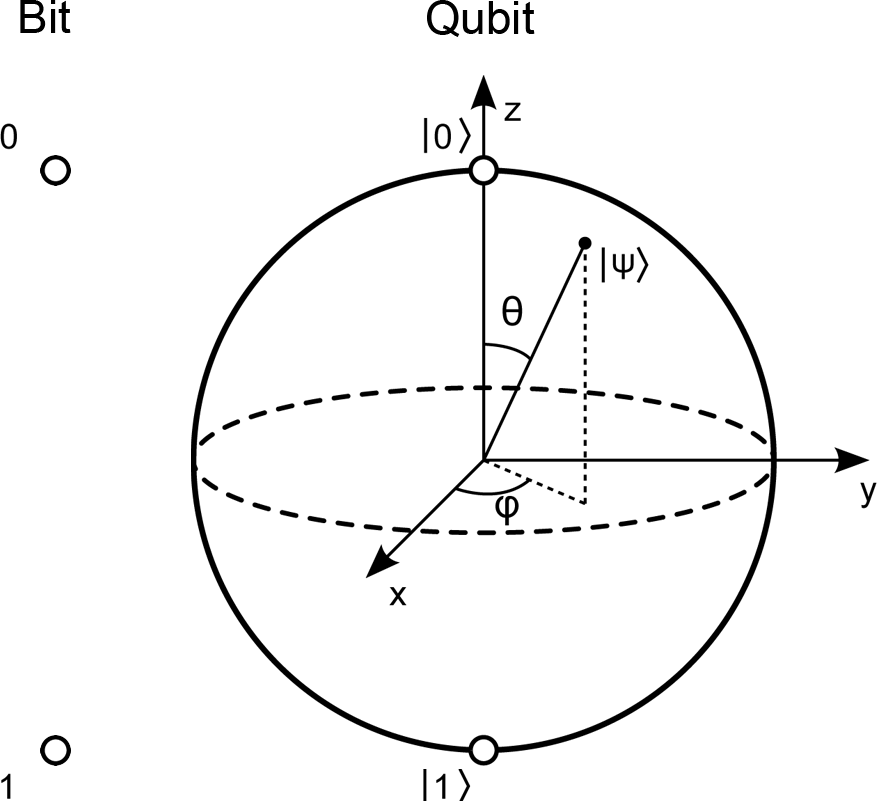
\includegraphics[width=0.4\textwidth]{bloch_sphere}
    \caption{A comparison of a bit and the Bloch sphere representation of a qubit.}
    \caption*{Modified, Meister 2009}
    \label{fig:bloch_sphere}
\end{figure}
A quantum computer leverages three key principles of quantum physics, or properties of quantum objects (atoms, ions and photons):
\begin{enumerate}
\item Superposition: the state in which a quantum object exists in multiple possible states simultaneously;
\item Interference: the possibility that the wave function of a particle will either destructively or constructively interfere with another particle’s wave function;
\item Entanglement: the connection between particles, resulting in an inability to determine the quantum state of an individual particle, without the other particle it is entangled to.
\citep{doi:10.1142/q0243}.
\end{enumerate}

\subsection{Artificial Neural Networks}
Artificial neural networks (ANN) are the basis of machine learning (ML) and artificial intelligence (AI) algorithms. ANNs attempt to simulate the human brain, replicating its structure with a web of interconnected nodes (artificial neurons). Biological neurons consist of dendrites (inputs), cell body which contains the nucleus (processing), and an axon which terminates as axon branches (outputs), and interlinked by electrical or chemical synapses. Nodes mimic this structure, as shown in figure \ref{fig:neuron}.
\begin{figure}[h]
    \centering
    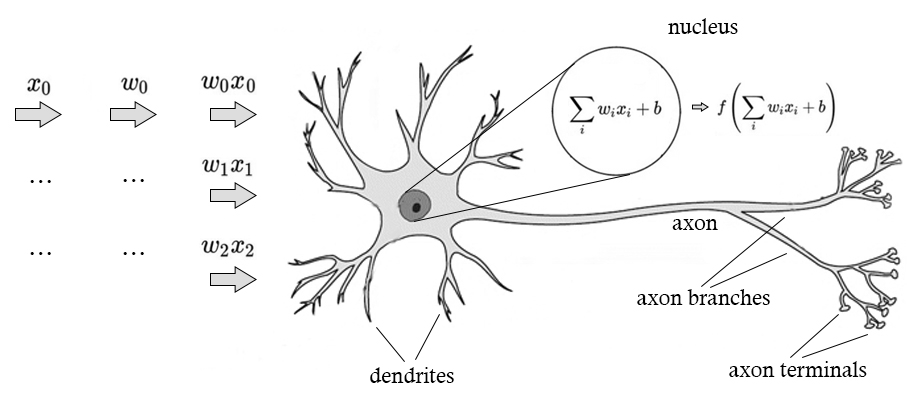
\includegraphics[width=0.8\textwidth]{neuron}
    \caption{A biological neuron, labelled with an artificial neuron's properties.}
    \caption*{Modified, Bolton 2018}
    \label{fig:neuron}
\end{figure}
Fundamentally, a node is a function. Inputs (for example, x\textsubscript{0}) are modified by a scalar weight variable (in the instance of x\textsubscript{0}, w\textsubscript{0}) to control the influence of each input. The total influence (sum of all weighted inputs) is then input into an activation function (figure \ref{fig:activation_functions}), which like a biological neuron's activation potential, will trigger the neuron to 'fire' if above the threshold (bias). Shown in figure \ref{fig:neuron}, the summation process can be described by
\begin{equation}
     \sum_{i}^{}w_ix_i+b
\end{equation}
\emph{where w\textsubscript{i} is the weight of the i\textsuperscript{th} neuron, x\textsubscript{i} is the input of the i\textsuperscript{th} neuron, and b is the bias}. Weights and bias are adjusted for optimal task-specific performance during the training of a network.
\begin{figure}[h]
    \centering
    \begin{subfigure}[t]{0.4\textwidth}
    	\begin{tikzpicture}
			\begin{axis}[width=6cm,height=6cm,ylabel=$f(x)$,xlabel=$x$,ymin=-0.2,ymax=1,xmin=-5,xmax=5]
				\addplot[black,smooth] {1/(1+exp(-x))} node[] at (2.5, 0.3) {$f(x)=\frac{1}{1+e^{-x}}$};
			\end{axis}
		\end{tikzpicture}
        \caption{Logistic sigmoid.}
    \end{subfigure}
    \begin{subfigure}[t]{0.4\textwidth}
    	\begin{tikzpicture}
			\begin{axis}[width=6cm,height=6cm,ylabel=$f(x)$,xlabel=$x$,ymin=-0.2,ymax=1,xmin=-5,xmax=5]
				\addplot+[mark=none,black,domain=-5:0] {0};
                \addplot+[mark=none,black,domain=0:5] {x} node[] at (0, -0.1) {$f(x)=\begin{array}{rcl} 0 & \mbox{for} & x < 0\\ x & \mbox{for} & x \ge 0\end{array}$};
			\end{axis}
		\end{tikzpicture}
        \caption{ReLU.}
    \end{subfigure}
    \caption{Activation functions.}
    \label{fig:activation_functions}
\end{figure}
A simple feed-forward neural network (FFNN) is illustrated in figure \ref{fig:net}: nodes are arranged in layers, each independent of its vertical nodes but interconnected with every horizontal node in other layers. The first layer is the input layer, the layers between are hidden layers, and the last layer is the output layer.
\begin{figure}[htp]
    \centering
    \begin{neuralnetwork}[height=5]
        \newcommand{\x}[2]{$x_#2$}
        \newcommand{\y}[2]{$\hat{y}_#2$}
        \newcommand{\hfirst}[2]{\small $h^{(1)}_#2$}
        \newcommand{\hsecond}[2]{\small $h^{(2)}_#2$}
        \inputlayer[count=4, bias=true, title=Input\\layer, text=\x]
        \hiddenlayer[count=3, bias=false, title=Hidden\\layer\\(quantum), text=\hfirst] \linklayers
        \outputlayer[count=2, title=Output\\layer, text=\y] \linklayers
    \end{neuralnetwork}
    \caption{Representation of a simple neural network.}
    \label{fig:net}
\end{figure}

\subsection{Hybrid Quantum-Classical Neural Networks}
Due to the widespread nature of classification ANN, hybrid quantum-classical neural networks may prove most useful by enhancing feature spaces (increase the number of features used in the characterisation of data), as explored in \citep{Havlicek2019a}. Previous similar research, notably involving the implementation of classification QML models on quantum computers include \citep{Schuld2017}, \citep{Grant2018} and \citep{Tacchino2019}. Prior experimental research has sought to prove that QML is possible, whilst theoretical research has determined QML algorithms to be exponentially faster than classical algorithms \citep{Lloyd2013}.

Hybrid quantum-classical neural networks can be implemented using parameterised quantum circuits (PQCs), which take rotation angles related to the input vectors as input parameters. With current technical limitations, implementing PQCs as hidden layers in a simple FFNN is the simplest approach.

\newpage
\section{Research Question}
How is the classification accuracy of a hybrid quantum-classical neural network affected by the number of qubits in its hidden parameterised quantum circuit layer?

\section{Hypothesis}
As the number of qubits utilised increases, the accuracy of the neural network will decrease. Limitations on quantum computational power due to noise in the hardware is supported by \citep{preskill}.
\\+more justification to be added

\section{Methodology}
Open source code for a hybrid classical-quantum neural network was obtained from the \emph{Qiskit} textbook, and modified for the purpose of data collection and variable control (the modified code is available in appendix \ref{code}). The majority of prior research involving classification QML models had been conducted on IBM quantum computers with quantum processor based artificial neurons, and accuracy had been measured in simple pattern recognition tasks \citep{Benedetti2019}. Thus, the quantum circuit (figure \ref{fig:single_qubit_circ}, with all variations used available in appendix \ref{circuits}) was run on ibmq\_manila, an IBM quantum machine with a 5 qubit Falcon r5.11L processor and a quantum volume of 32. Five trials were conducted, each testing circuits utilising all numbers of qubits available (1, 2, 3, 4 and 5 qubits).
\begin{figure}[h]
    \centering
    \begin{equation*}
        \Qcircuit @C=1.0em @R=0.2em @!R {
                    \lstick{ {q}_{0} :  } & \gate{\mathrm{H}} \barrier[0em]{0} & \qw & \gate{\mathrm{R}_\mathrm{Y}\,\mathrm{(}\mathrm{\theta}\mathrm{)}} \barrier[0em]{0} & \qw & \meter & \qw & \qw\\
                    \lstick{meas:} & \lstick{/_{_{1}}} \cw & \cw & \cw & \cw & \dstick{_{_{0}}} \cw \cwx[-1] & \cw & \cw\\
        }
    \end{equation*}
    \caption{Single qubit variation of the circuit used.}
    \label{fig:single_qubit_circ}
\end{figure}
Variables are outlined below in table \ref{variables}.
\begin{center}
\begin{tabular}{ |c|c|c| }
\hline
Independent & Dependent & Controlled \\
\hline
{Number of qubits} & {Percent accuracy of neural network} & {Quantum computer (ibmq\_manila)} \\ 
&  & {Code utilised (hnn.py)} \\ 
&  & {Training and datasets} \\ 
\hline
\end{tabular}
\captionof{table}{Independent, dependant and controlled variables.} \label{variables}
\end{center}
Accuracy was measured using percent correct classification (PCC), a method which treated every error with the same weight \citep{Twomey1995}, resulting in a focus on the hybrid quantum-classical neural network’s effectiveness. Figure \ref{fig:T5Q5_Labels} shows a set of predictions with a PCC of 60\% (3 correct, 2 incorrect).
\begin{figure}[h]
    \centering
    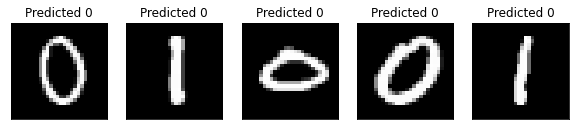
\includegraphics[width=0.8\textwidth]{T5Q5_Labels.png}
    \caption{Output labels.}
    \label{fig:T5Q5_Labels}
\end{figure}
\\+acknowledgement of possible errors: hardware noise contributing to erroneous results, training data set biases/overlap with testing data set resulting in very high/perfect classification accuracy
\newpage
\section{Results}
Data collection is still in progress. Currently there are 16 recorded accuracy values and 11 recorded loss values. The average of these values are in table \ref{avgresults}.
\begin{center}
\begin{tabular}[h]{ |c|c|c| }
\hline
Qubits & Accuracy & Loss\\
\hline
{1} & {44.88\%} & {-0.4995333333}\\ 
\hline
{2} & {50.00\%} & {-0.5168}\\
\hline
{3} & {50.00\%} & {-0.2936}\\ 
\hline
{4} & {50.00\%} & {3.04}\\ 
\hline
{5} & {50.00\%} & {-62.1343}\\ 
\hline
\end{tabular}
\captionof{table}{Average accuracy and loss for each number of qubits.} \label{avgresults}
\end{center}
-loss (just realised that it's not relevant)\\
Use of 1 qubit has the lowest accuracy of 44.88\%. Use of 2, 3, 4 and 5 qubits had equal accuracy of 50\%. Use of 3 qubits resulted in the smallest magnitude of error, 0.2936. Use of 5 qubits resulted in the greatest magnitude of error, 62.1343.
\\+histogram or scatter plot
\\+pearsons correlation, gradient of curve

\section{Discussion}
The single qubit system having the lowest accuracy was unexpected. All other qubit value systems having equal accuracy indicates a systematic error.
\\+little to no relationship due to low pearsons (i assume?)
\\+errors: too few training epochs resulting in weak model (systematic), hardware noise resulting in erroneous results (random), binary options with even number of test images likely resulted in consistent 50\% accuracy
\\+future recommendations: changing of more variables (epoch, training data, activation function) to focus more on the quantum layer's impact

\section{Conclusion}
+research question was addressed - variable control resulted in high validity
\\+key findings, currently -> did not support the hypothesis -> reasons for this

\newpage

\bibliography{references}

\newpage

\appendix
\renewcommand{\thesection}{\Alph{section}.\arabic{section}}
\begin{appendices}
\section{Code}
\label{code}
\inputminted{octave}{code/hnn.py}
\newpage
\section{Circuits}
\label{circuits}
\subsection{1 Qubit}
\begin{equation*}
    \Qcircuit @C=1.0em @R=0.2em @!R {
                \lstick{ {q}_{0} :  } & \gate{\mathrm{H}} \barrier[0em]{0} & \qw & \gate{\mathrm{R}_\mathrm{Y}\,\mathrm{(}\mathrm{\theta}\mathrm{)}} \barrier[0em]{0} & \qw & \meter & \qw & \qw\\
                \lstick{meas:} & \lstick{/_{_{1}}} \cw & \cw & \cw & \cw & \dstick{_{_{0}}} \cw \cwx[-1] & \cw & \cw\\
         }
\end{equation*}
\subsection{2 Qubit}
\begin{equation*}
    \Qcircuit @C=1.0em @R=0.2em @!R {
                \lstick{ {q}_{0} :  } & \gate{\mathrm{H}} \barrier[0em]{1} & \qw & \gate{\mathrm{R}_\mathrm{Y}\,\mathrm{(}\mathrm{\theta}\mathrm{)}} \barrier[0em]{1} & \qw & \meter & \qw & \qw & \qw\\
                \lstick{ {q}_{1} :  } & \gate{\mathrm{H}} & \qw & \gate{\mathrm{R}_\mathrm{Y}\,\mathrm{(}\mathrm{\theta}\mathrm{)}} & \qw & \qw & \meter & \qw & \qw\\
                \lstick{meas:} & \lstick{/_{_{2}}} \cw & \cw & \cw & \cw & \dstick{_{_{0}}} \cw \cwx[-2] & \dstick{_{_{1}}} \cw \cwx[-1] & \cw & \cw\\
         }
\end{equation*}
\subsection{3 Qubit}
\begin{equation*}
    \Qcircuit @C=1.0em @R=0.2em @!R {
                \lstick{ {q}_{0} :  } & \gate{\mathrm{H}} \barrier[0em]{2} & \qw & \gate{\mathrm{R}_\mathrm{Y}\,\mathrm{(}\mathrm{\theta}\mathrm{)}} \barrier[0em]{2} & \qw & \meter & \qw & \qw & \qw & \qw\\
                \lstick{ {q}_{1} :  } & \gate{\mathrm{H}} & \qw & \gate{\mathrm{R}_\mathrm{Y}\,\mathrm{(}\mathrm{\theta}\mathrm{)}} & \qw & \qw & \meter & \qw & \qw & \qw\\
                \lstick{ {q}_{2} :  } & \gate{\mathrm{H}} & \qw & \gate{\mathrm{R}_\mathrm{Y}\,\mathrm{(}\mathrm{\theta}\mathrm{)}} & \qw & \qw & \qw & \meter & \qw & \qw\\
                \lstick{meas:} & \lstick{/_{_{3}}} \cw & \cw & \cw & \cw & \dstick{_{_{0}}} \cw \cwx[-3] & \dstick{_{_{1}}} \cw \cwx[-2] & \dstick{_{_{2}}} \cw \cwx[-1] & \cw & \cw\\
         }
\end{equation*}
\subsection{4 Qubit}
\begin{equation*}
    \Qcircuit @C=1.0em @R=0.2em @!R {
                \lstick{ {q}_{0} :  } & \gate{\mathrm{H}} \barrier[0em]{3} & \qw & \gate{\mathrm{R}_\mathrm{Y}\,\mathrm{(}\mathrm{\theta}\mathrm{)}} \barrier[0em]{3} & \qw & \meter & \qw & \qw & \qw & \qw & \qw\\
                \lstick{ {q}_{1} :  } & \gate{\mathrm{H}} & \qw & \gate{\mathrm{R}_\mathrm{Y}\,\mathrm{(}\mathrm{\theta}\mathrm{)}} & \qw & \qw & \meter & \qw & \qw & \qw & \qw\\
                \lstick{ {q}_{2} :  } & \gate{\mathrm{H}} & \qw & \gate{\mathrm{R}_\mathrm{Y}\,\mathrm{(}\mathrm{\theta}\mathrm{)}} & \qw & \qw & \qw & \meter & \qw & \qw & \qw\\
                \lstick{ {q}_{3} :  } & \gate{\mathrm{H}} & \qw & \gate{\mathrm{R}_\mathrm{Y}\,\mathrm{(}\mathrm{\theta}\mathrm{)}} & \qw & \qw & \qw & \qw & \meter & \qw & \qw\\
                \lstick{meas:} & \lstick{/_{_{4}}} \cw & \cw & \cw & \cw & \dstick{_{_{0}}} \cw \cwx[-4] & \dstick{_{_{1}}} \cw \cwx[-3] & \dstick{_{_{2}}} \cw \cwx[-2] & \dstick{_{_{3}}} \cw \cwx[-1] & \cw & \cw\\
         }
\end{equation*}
\subsection{5 Qubit}
\begin{equation*}
    \Qcircuit @C=1.0em @R=0.2em @!R {
                \lstick{ {q}_{0} :  } & \gate{\mathrm{H}} \barrier[0em]{4} & \qw & \gate{\mathrm{R}_\mathrm{Y}\,\mathrm{(}\mathrm{\theta}\mathrm{)}} \barrier[0em]{4} & \qw & \meter & \qw & \qw & \qw & \qw & \qw & \qw\\
                \lstick{ {q}_{1} :  } & \gate{\mathrm{H}} & \qw & \gate{\mathrm{R}_\mathrm{Y}\,\mathrm{(}\mathrm{\theta}\mathrm{)}} & \qw & \qw & \meter & \qw & \qw & \qw & \qw & \qw\\
                \lstick{ {q}_{2} :  } & \gate{\mathrm{H}} & \qw & \gate{\mathrm{R}_\mathrm{Y}\,\mathrm{(}\mathrm{\theta}\mathrm{)}} & \qw & \qw & \qw & \meter & \qw & \qw & \qw & \qw\\
                \lstick{ {q}_{3} :  } & \gate{\mathrm{H}} & \qw & \gate{\mathrm{R}_\mathrm{Y}\,\mathrm{(}\mathrm{\theta}\mathrm{)}} & \qw & \qw & \qw & \qw & \meter & \qw & \qw & \qw\\
                \lstick{ {q}_{4} :  } & \gate{\mathrm{H}} & \qw & \gate{\mathrm{R}_\mathrm{Y}\,\mathrm{(}\mathrm{\theta}\mathrm{)}} & \qw & \qw & \qw & \qw & \qw & \meter & \qw & \qw\\
                \lstick{meas:} & \lstick{/_{_{5}}} \cw & \cw & \cw & \cw & \dstick{_{_{0}}} \cw \cwx[-5] & \dstick{_{_{1}}} \cw \cwx[-4] & \dstick{_{_{2}}} \cw \cwx[-3] & \dstick{_{_{3}}} \cw \cwx[-2] & \dstick{_{_{4}}} \cw \cwx[-1] & \cw & \cw\\
         }
\end{equation*}
\end{appendices}
\end{document}
